%\documentclass[12pt,landscape]{article}
%\usepackage{tikz}
%\usetikzlibrary{positioning}
%\usetikzlibrary{fit,shapes.geometric}
%\usetikzlibrary{calc}
%\usepackage{amsfonts}
%\usepackage{amsmath, amsthm, amssymb}
%\usepackage{verbatim}

%\usepackage[active, tightpage]{preview} % used to crop file size to image size
%\setlength\PreviewBorder{0pt}%
%\begin{document}
%\begin{preview}
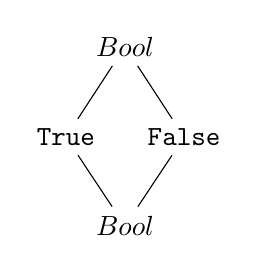
\begin{tikzpicture}[node distance=1.8cm]
  %\draw [help lines, dotted] (-8,1) grid (8,-10);

  %\node(Top)   {$\Top{Value}$};
  %\node(Bot)   [below=6cm of Top] {$\Bot{Value}$};
  %\path node (center) at ($.5*(Top) + .5*(Bot)$) {};
  %\path node (center) at (0,0) {};

  %\path node (bool)    at ([xshift=-4.2cm, yshift= 11.4mm] center) {};
  \path node (bool)    at (0,0) {};
  %\path node (int)     at ([xshift=-0.8cm, yshift= 11.4mm] center) {};
  %\path node (float)   at ([xshift= 2.4cm, yshift= 11.4mm] center) {};
  %\node(None)          at ([xshift= 5.2cm] center) {\texttt{None}};
  %\node(Undefined)     at ([xshift= 5.4cm] center) {\texttt{Undefined}};
  %\path node (list)    at ([xshift= 7.1cm, yshift= 11.4mm] center) {};
  %\node                at ([xshift= 5.8cm] center) {$\cdots$};
  %\path node (sep)     at ([xshift= 7.4cm] center) {};
  %\path node (nparray) at ([xshift= 9.1cm, yshift= 11.4mm] center) {};

  %\node                at ([xshift= 5.3cm, yshift=-3.0cm] center) {Built-ins};
  %\node                at ([xshift= 7.8cm, yshift=-3.0cm] center) {User defined};

  \node(TopBool)  at (bool)                     {$\Top{Bool}$};
  \node(BotBool)  at ([yshift=-22.8mm] TopBool) {$\Bot{Bool}$};
  \node(True)     at ([xshift=-.75cm, yshift=-1.15cm] TopBool)   {\texttt{True}};
  \node(False)    at ([xshift= .75cm, yshift=-1.15cm] TopBool)  {\texttt{False}};
  %\node[ellipse, dotted, draw, thick, fit=(TopBool) (BotBool) (True) (False), inner sep=-3.3mm] {};
  \foreach \x in {True,False} {
    \draw(TopBool) -- (\x);
    \draw(BotBool) -- (\x);
  }
  %\draw(Top) -- (TopBool);
  %\draw(Bot) -- (BotBool);

  %\node(TopInt) at (int)       {$\Top{Int}$};
  %\node(i0)     at ([xshift=-1.5cm, yshift=-1.15cm] TopInt)   {0};
  %\node(i1)     at ([xshift=-.75cm, yshift=-1.15cm] TopInt)   {1};
  %\node(i4232)  at ([xshift=  .3cm, yshift=-1.15cm] TopInt)   {4232};
  %\node(idots)  at ([xshift= 1.5cm, yshift=-1.15cm] TopInt)   {$\cdots$};
  %\node(BotInt)  [below=1.6cm of TopInt]                 {$\Bot{Int}$};
  %\node[ellipse, dotted, draw, thick, fit=(TopInt) (BotInt) (i0) (idots),
  %      inner ysep=-3mm, inner xsep=-5.5mm] {};
  %\foreach \x in {i0,i1,i4232,idots} {
  %  \draw(TopInt) -- (\x);
  %  \draw(BotInt) -- (\x);
  %}
  %\draw(Top) -- (TopInt);
  %\draw(Bot) -- (BotInt);

  %\node(TopFloat)  at (float) {$\Top{Float}$};
  %\node(BotFloat)  at ([yshift=-22.8mm] TopFloat) {$\Bot{Float}$};
  %\node(Float)     at ([yshift=-11.4mm] TopFloat) {\textit{Float}};
  %\draw(Top) -- (TopFloat);
  %\draw(Bot) -- (BotFloat);
  %\node[ellipse, dotted, draw, thick, fit=(TopFloat) (BotFloat), inner sep=-3mm, inner xsep=2mm] {};

  %\draw(Top) -- (None);
  %\draw(Bot) -- (None);

  %\draw(Top) -- (Undefined);
  %\draw(Bot) -- (Undefined);

  % \node(TopList)  at (list) {$\top_{\hspace{-1mm}{\text{\tiny{List}}}}$};
  % \node(BotList)  at ([yshift=-22.8mm] TopList) {$\bot_{\text{\tiny{List}}}$};
  % \node(List)     at ([yshift=-11.4mm] TopList) {\textit{List}};
  % \draw(Top) -- (TopList);
  % \draw(Bot) -- (BotList);
  % \node[ellipse, dotted, draw, thick, fit=(TopList) (BotList), inner sep=-3mm, inner xsep=2mm] {};

  % \node(upsep)    at ([yshift=-3.5cm] sep) {};
  % \node(downsep)  at ([yshift= 3.5cm] sep) {};
  % \draw[dotted, thick](upsep) -- (downsep);

  % \node(TopArray)  at (nparray) {$\top_{\hspace{-1mm}{\text{\tiny{NPArray}}}}$};
  % \node(BotArray)  at ([yshift=-22.8mm] TopArray) {$\bot_{\text{\tiny{NPArray}}}$};
  % \node(List)     at ([yshift=-11.4mm] TopArray) {\textit{NPArray}};
  % \draw(Top) -- (TopArray);
  % \draw(Bot) -- (BotArray);
  % \node[ellipse, dotted, draw, thick, fit=(TopArray) (BotArray), inner sep=-3mm, inner xsep=2mm] {};

\end{tikzpicture}
%\end{preview}
%\end{document}
